\documentclass[10pt]{beamer}
\usetheme{CambridgeUS}
\usepackage{amsmath}
\usepackage{amsfonts}
\usepackage{amsthm}
\usepackage{amssymb}
\usepackage{subfig}
\usepackage{tikz}
\usepackage{tabu}
\usepackage{booktabs}

\definecolor{cof}{RGB}{219,144,71}
\definecolor{pur}{RGB}{186,146,162}
\definecolor{greeo}{RGB}{91,173,69}
\definecolor{greet}{RGB}{52,111,72}


\usepackage[utf8]{inputenc}


%Information to be included in the title page:
\title{Log-concave Sampling (Part 1)}
\author{Marios Papachristou}
\institute{GeomScale, NTUA}
\date{\today}

\begin{document}

\begin{frame}
    \titlepage
    \begin{center}
        
\includegraphics[width=0.3\textwidth]{publications/presentations/log_concave_sampling/logo.png} \quad 
        
\includegraphics[width=0.1\textwidth]{publications/presentations/log_concave_sampling/gsoc.png} \quad
        
\includegraphics[width=0.25\textwidth]{publications/presentations/log_concave_sampling/cc.png}
    \end{center}
    
    \small {
    Mentors: A. Chalkis (NKUA), V. Fisikopoulos (NKUA), E. Tsigaridas (INRIA) \\
    Homepage: \url{https://github.com/GeomScale/volume_approximation} 
    }
\end{frame}


\begin{frame}{About today's talk / tutorial}

Today's talk will concentrate on 
\\
\textbf{Sampling from high-dimensional log-concave densities}

\begin{enumerate}
    \item Introduction to log-concave sampling.
    \item ODE Solvers.
    \item Boundary Oracles.
\end{enumerate}


\end{frame}

\begin{frame}{Google Summer of Code 2020}

The current GSoC project aims to provide implementations (and theoretical insights) to log-concave sampling problems for the GeomScale project.

Milestones 

\begin{enumerate}
    \item Milestone I (ODE Solvers)
    \begin{itemize}
        \item Implement ODE solvers (Euler, Runge-Kutta, Collocation, etc.)
        \item Efficiently address boundary oracles
    \end{itemize}
    \item Milestone II (Samplers) 
    \begin{itemize}
        \item Implement samplers (HMC, Langevin etc.).  
        \item Provide theoretical guarantees on truncated settings. 
    \end{itemize}
    
    \item Milestone III (R bindings)
    \begin{itemize}
        \item Port C++ functionality of 
    \end{itemize}
    
    
    Today's talk will mostly concentrate on \textbf{Milestone I}.
    
\end{enumerate}


    
\end{frame}

\begin{frame}{Basics}
    Our project involves taking samples from distributions with probability density functions of the form
    
    $$\pi(x) \propto \exp(-f(x)) \qquad x \in K$$ 
    
    where $K$ is either: (a) $\mathbb R^d$, or (b) a convex body, and $f$ is a convex function that is $L$-smooth and $m$-strongly convex. 

\end{frame}

\begin{frame}[allowframebreaks]{Convex Functions}

A domain $K$  is convex iff (if and only if) for all $x, y \in K$ it holds that for all $t \in [0, 1]$ 

$$tx + (1-t)y \in K$$

The domain $K$ is a convex body iff it is convex, closed and bounded. 

A function $f: K \to \mathbb R$ is convex iff for all $x, y \in K$ we have that for all $t \in [0, 1]$

$$
    f(tx + (1-t)y) \le t f(x) + (1-t) f(y)
$$

Convex functions have some very nice properties, and their use is widespread in optimization.  
    
\framebreak    
    

\begin{figure}[t]
    \centering
    \subfloat[$L^1$-ball]{
    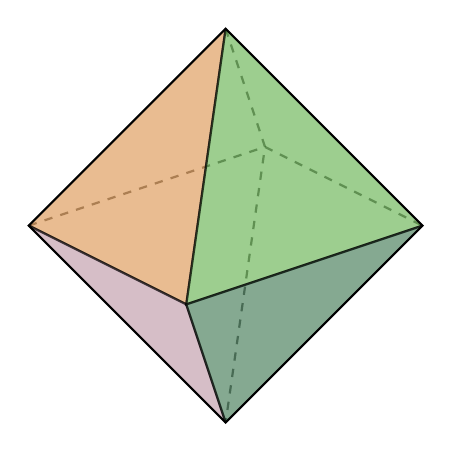
\begin{tikzpicture}[thick,scale=5]
    \coordinate (A1) at (0,0);
    \coordinate (A2) at (0.6,0.2);
    \coordinate (A3) at (1,0);
    \coordinate (A4) at (0.4,-0.2);
    \coordinate (B1) at (0.5,0.5);
    \coordinate (B2) at (0.5,-0.5);
    
    \begin{scope}[thick,dashed,,opacity=0.6]
    \draw (A1) -- (A2) -- (A3);
    \draw (B1) -- (A2) -- (B2);
    \end{scope}
    \draw[fill=cof,opacity=0.6] (A1) -- (A4) -- (B1);
    \draw[fill=pur,opacity=0.6] (A1) -- (A4) -- (B2);
    \draw[fill=greeo,opacity=0.6] (A3) -- (A4) -- (B1);
    \draw[fill=greet,opacity=0.6] (A3) -- (A4) -- (B2);
    \draw (B1) -- (A1) -- (B2) -- (A3) --cycle;
    \end{tikzpicture}
    } \qquad
    \subfloat[$L^2$-ball]{
    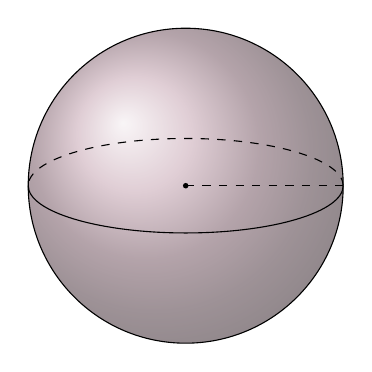
\begin{tikzpicture}
    \shade[ball color = pur, opacity = 0.6] (0,0) circle (2cm);
    \draw (0,0) circle (2cm);
    \draw (-2,0) arc (180:360:2 and 0.6);
    \draw[dashed] (2,0) arc (0:180:2 and 0.6);
    \fill[fill=black] (0,0) circle (1pt);
    \draw[dashed] (0,0 ) -- node[above]{} (2,0);
    \end{tikzpicture}
    }
    \caption{Examples of convex bodies.}
    \label{fig:examples}
\end{figure}
    
    
\framebreak    
    
If the function is twice differentiable with gradient $\nabla f$ and Hessian matrix $\nabla^2 f$ then
\begin{itemize}
    \item We say that $f$ is $L$-smooth iff $\| \nabla f(x) - \nabla f(y) \| \le L \| x - y \|$ or $\nabla^2 f(x) \preceq L \cdot I_d$.
    \item We say that $f$ is $m$-strongly convex iff 
    $$f(y) \ge f(x) + \langle \nabla f(x), y - x \rangle + \frac m 2 \| x - y \|^2 $$
    
    or $\nabla^2 f(x) \succeq m \cdot I_d$.
    
    \item The above generalize in a looser setting as well.     
    
    \item We define the \textbf{condition number} of $f$ to be the ratio of max/min eigenvalues of the Hessian, that is $\kappa = L / m$.
    
\end{itemize}
\end{frame}

\begin{frame}[allowframebreaks]{Random Walks and Sampling}

    Our goal is sampling from $\pi(x) \propto \exp(-f(x))$. 
    
    \medskip
    
    Directly sampling from $\pi(x)$ is very difficult since one has to account for the normalization constant $\int_K \exp(-f(x)) d x$ which is in general \textbf{intractable}. 
    
    \medskip
    
    \textbf{Idea.} The distribution $\pi(x)$ can be thought as the stationary measure of a Markov Chain that is $\pi(x) = \lim_{k \to \infty} \pi_k(x)$. 

    \medskip

    The dependence on the dimension $d$ and the condition number $\kappa$ of $f$ are interesting.
    
    \framebreak
    
    One of the first algorithms to do it is the Metropolis-Hastings Algorithm. The general idea of Metropolis Hastings is 
    
    \begin{enumerate}
        \item Assume that you are at a state $x$ 
        \item Perform a transition to a new nearby state $y$ and make a proposal for transitioning to $y$
        \item Accept the proposal to move to $y$ with probability (Metropolis Filter)
        
        $$\min \left  \{ 1, \frac { a (x, y) \pi(y) } {a (y, x) \pi (x)} \right \}$$
        
        where $a$ is a transition probability function. 
        
    \end{enumerate}
    
    It can be shown analytically that the above process converges to a stationary distribution $\pi(x)$.
    
    \textbf{Intuition when $a(x,y) = a(y,x)$:} The sampler has incentive to move towards higher-density areas (but lower density areas are also allowed)
    
\end{frame}



\begin{frame}[allowframebreaks]{Algorithmic Challenges}

The main Algorithmic Challenges for (log-concave) sampling are in general

\begin{enumerate}
    \item The \textbf{Mixing Time} of the Markov Chain, that is how fast (\# iterations) a Markov Chain with transition operator $\mathcal T$ starting from an initial distribution $\pi_0$ reaches $\pi$ within Total Variation Distance of at most $\delta > 0$ (more next time)
    
    $$t_{mix}(\delta) = \inf \left \{ k \ge 0 | \| \mathcal T^k (\pi_0) - \pi \|_{TV} \le \delta \right \}$$
    
    where $\| P - Q \|_{TV} = \sup_{A \in \mathcal F} |P(A) - Q(A)|$ and $\mathcal F$ is a $\sigma$-algebra on the state space $K$. 
    
    \item The \textbf{Cost-Per Iteration} that is 
    
    $$\binom {\text {Cost-per}} {\text{iteration}} = \binom {\text {Cost-per}} {\text{ODE step}} + \binom {\text {Cost-per boundary}} {\text{oracle (if truncated)}}$$

    \end{enumerate}


    \framebreak
    
        
    \begin{table}
        \centering
        \begin{tabu} to \textwidth {X[3] X X[3] X}
        \toprule
            Method & Support & Mixing Time & Distance \\
        \midrule
            MALA/HMC \cite{dwivedi2019log} & $\mathbb R^d$ &  $\tilde O(\max \{ \kappa d, \kappa^{1.5} \sqrt d \})$ & TVD \\
            MALA/HMC \cite{lee2020logsmooth} & $\mathbb R^d$ & $\tilde O(\kappa d)$ & TVD \\
            ULD \cite{shen2019randomized} & $\mathbb R^d$ & $\tilde O(\kappa^{7/6} / \epsilon^{1/3} + \kappa / \epsilon^{2/3}) $ & $\mathcal W_2$ \\
            Our conjecture (log-concave) & $K$  & $\tilde O(\kappa d)$ & TVD \\
            \midrule 
            Coord. Hit-and-Run \cite{haraldsdottir2017chrr} &  $K$ & $O(d^2)$ & TVD \\
            Our conjecture (Billiard) & $K$ & $\tilde O(d)$ & TVD \\
        \bottomrule
        \end{tabu}
        \caption{Known results for the mixing time of random-walk methods. Above: First-order Methods. Below: Zero-order Methods. $K$ is a convex body. The notation $\tilde O(\cdot)$ ignores logarithmic factors. The logarithmic factors (in the case of convex-body support) depend on the condition number and the ``shape'' of the polytope.}
        \label{table:methods}
    \end{table}

    



    
\end{frame}

\begin{frame}
    \vfill 
    \centering
    \Large
    \textbf{Sampling in a continuous setting}
    \vfill
\end{frame}


\begin{frame}[allowframebreaks]{Hamiltonian Monte Carlo}
    
    The state-space is continuous and the samples can be proposed via solving Hamilton's equations for a particle with position $x$ and velocity $v$ under a conservative potential $f(x)$ that applies a force $-\nabla f(x)$. \cite{duane1987hybrid}
    
    The Hamiltonian of the particle is defined as 
    
    \begin{equation*}
        H(x, v) = \color{red}{\underbrace{\frac 1 2 \| v \|^2}_{\text{kinetic energy}}} + \color{blue}{\underbrace{f(x)}_{\text{potential energy}}}
        
    \end{equation*}
    
    \begin{figure}
        \centering
        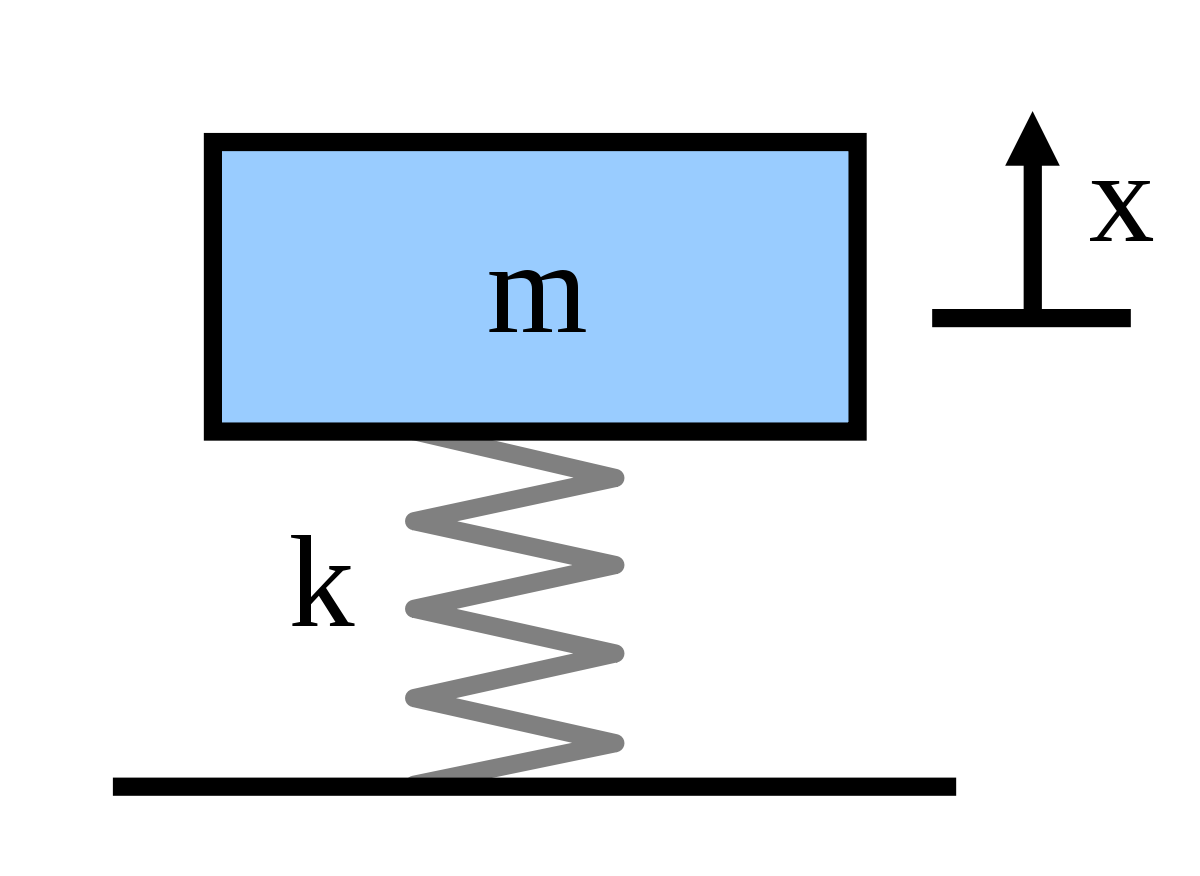
\includegraphics[ width=0.4\textwidth]{publications/presentations/log_concave_sampling/mass_spring.png}
        \caption{1D Mass-Spring System with mass $m = 1$ and spring constant $k = 1$ has a Hamiltonian $H(x, v) = \frac 1 2  v^2 + \frac 1 2 x^2$}
        \label{fig:my_label}
    \end{figure}
    
    \framebreak
    
     Hamilton's equations simulate the particle's behaviour in the conservative field
    
    \begin{align*}
        \dot x & = \frac {\partial H} {\partial v} =  v \\
        \dot v & = - \frac {\partial H} {\partial x} =  - \nabla f(x)
    \end{align*}
    
    \medskip
    
    In our previous example $\dot x = v$ and $\dot v = - x$ that is $\ddot x + x = 0$ which gives rise to the well-known simple harmonic oscilator $x(t) = A \cos (\omega t + \phi)$ 
    
    \framebreak
    
    We start by choosing a direction $v \sim \mathcal N(0, I_d)$ and simulate one/many steps of the ODE arriving at a proposal $(\tilde x, \tilde v)$. 
    
    \medskip
    
    The Metropolis Filter in this case for a proposal $(\tilde x, \tilde v)$ given a state $(x, v)$ is $\min \left \{ 1, \exp( H(\tilde x, \tilde v) - H(x, v) ) \right \}$.
    
    \medskip
    
    Ideally (i.e. with infinite precision) note that $\dot H = \langle \nabla_{x, v} H, (\dot x, \dot v) \rangle = \langle (v, \nabla f(x)), (- \nabla f(x), v) \rangle = 0$ and hence the Metropolis probability is always 1. 
    
    \medskip
    
    \textbf{However}, the ODE must be discretized and the \textbf{discretization error} makes the decision non-trivial. 
    
    \framebreak
    
    \textbf{Correctness.} The ODE admits a separable stationary measure proportional to
    
    $$\pi(x, v) \propto \exp(-H(x,v))$$
    
    The marginal density with respect to $x$ is therefore
    
    $$\pi(x) = \int_{\mathbb R^d} \pi(x, v) d v \propto \exp(-f(x))$$
    
    Hence the sequence of samples $x_1, \dots, x_i, \dots$ that the algorithm produces are $\epsilon$-close (in total variation distance) from the distribution $\pi(x)$. We need to make sure that the chain has ``mixed'' before ``trusting'' the samples.
    
    \framebreak
    
    \begin{figure}
        \centering
        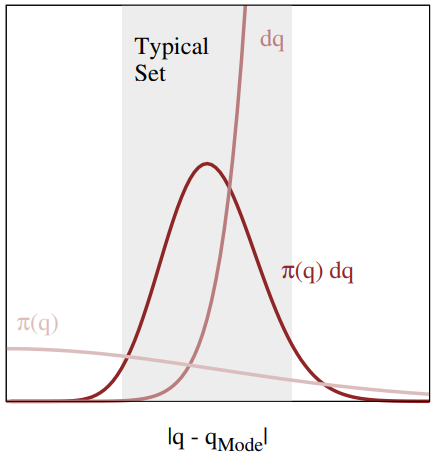
\includegraphics[width=0.5\textheight]{publications/presentations/log_concave_sampling/typical_1.png} \quad
        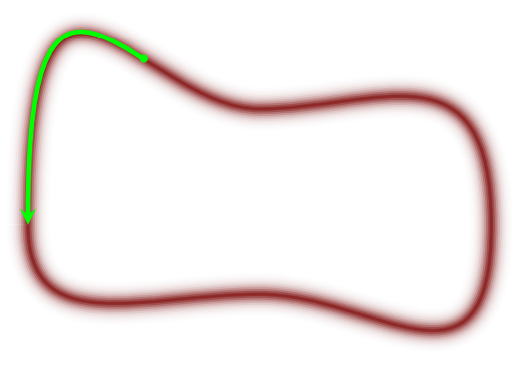
\includegraphics[width=0.5\textheight]{publications/presentations/log_concave_sampling/typical_path.png}
        \caption{The typical set of a Markov Chain. Formally, the typical path is defined the set of points $x$ where the product $\pi(x) dx $ is concentrated  }
        \label{fig:my_label}
    \end{figure}
    
    \framebreak
    
    \begin{figure}
        \centering
        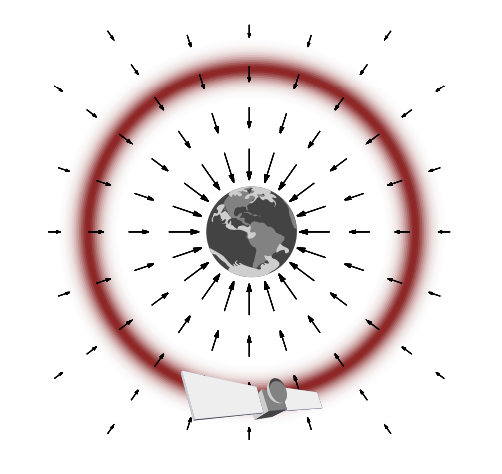
\includegraphics[width=0.4\textwidth]{publications/presentations/log_concave_sampling/satelite.png} \quad
         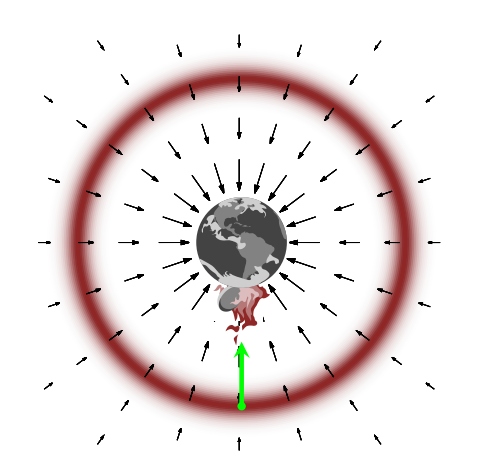
\includegraphics[width=0.4\textwidth]{publications/presentations/log_concave_sampling/crushing.png}
        \caption{Intuition behind HMC Sampling from \cite{betancourt2017conceptual}. Left: The vector field of $f$ is pointing towards the minimizer of $f$, that is $x^*$. The goal of the sampler (satelite) is to move on the red trajectory where the running sample mean approaches the expected value of $x$, that is $\mathbb E_{\pi} [x]$. Right: A gradient-inspired method (steepest descent $\dot x = - \nabla f(x)$) fails to maintain orbit around Earth (minimizer) and crushes into it.}
        \label{fig:my_label}
    \end{figure}
    
    \framebreak
    
    \begin{figure}
        \centering
        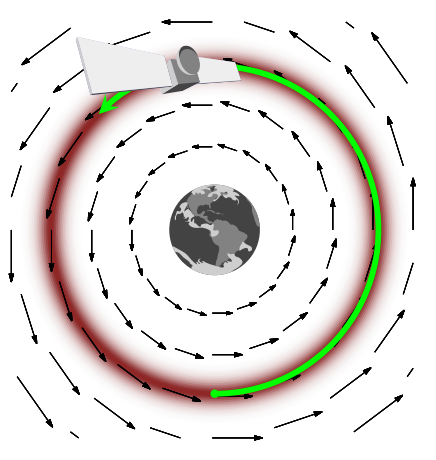
\includegraphics[height=0.4\textheight]{publications/presentations/log_concave_sampling/hmc.png} \quad
        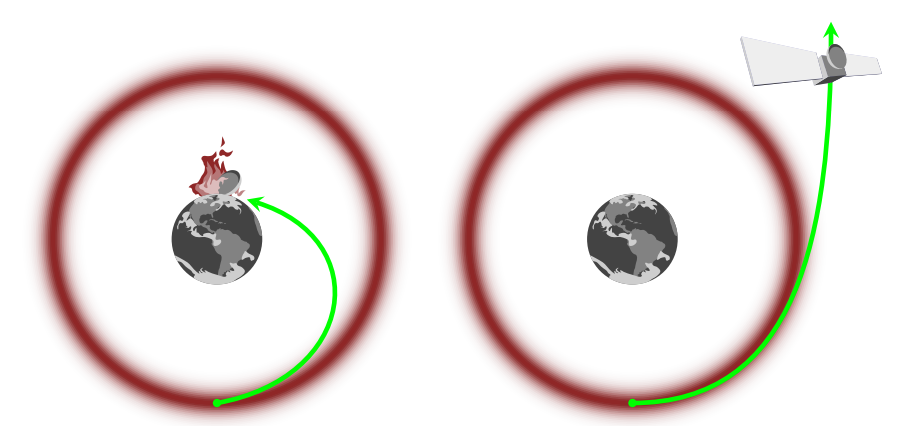
\includegraphics[height=0.4\textheight]{publications/presentations/log_concave_sampling/bad_trajectories.png}
        \caption{\textbf{HMC Idea. (Left)} The position $x$ of the sampler (orbiter) is corrected with a momentum term $v$ that counteracts the effects of ``gravity'' and keeps the sampler into orbit. 
        The HMC equations $\dot x = v$ and $\dot v = -\nabla f(x)$ assist the satelite to maintain orbit. 
        Middle: Adding too little momentum and the satelite crushes to the center again. Right: Adding to much momentum acts like a slingshot.  }
        \label{fig:my_label}
    \end{figure}
    
\end{frame}
    
\begin{frame}[allowframebreaks]{Langevin Dynamics}
    Another method for sampling is via solving the Langevin Stochastic Differential Equation which is the Newton's Second Law together with a Brownian Motion $W$. 
    
    \begin{align*}
        \dot x &= v \\
        \dot v &= - \gamma v - \nabla f(x) + \sqrt {2 \epsilon \gamma} \dot W
    \end{align*}
   
    where $\dot W$ is the derivative of the Brownian motion, that is $d W \sim \mathcal N(0, dt)$. Under mild conditions the SDE accepts a stationary measure proportional to $\exp \left ( - \frac 1 2 \| v \|^2  - f(x) \right )$. The parameters $\gamma$ (damping factor), $\epsilon$ determine the nature of the dynamics
    
    \begin{enumerate}
        \item when $\gamma > 1$ the system is overdamped (OLD equation)
        \item when $\gamma < 1$ the system is underdamped (ULD equation)
        \item when $\gamma = 1$ the system is critically damped
    \end{enumerate}

    \framebreak
    
    Of particular interest is the ULD equation
    
    \begin{align*}
        \dot x & = v \\
        \dot v & = -2v - u \nabla f(x) + 2 \sqrt u \dot W \\
        u & = 1 / L
    \end{align*}
    
    which is widely used in log-concave sampling. (for more information see \cite{lee2020logsmooth, lee2018algorithmic, gryazina2014random}). 
    
\end{frame}

\begin{frame}[allowframebreaks]{Sampling Applications}

\begin{enumerate}
    \item Integral Calculation (Monte-Carlo Integration)
    \item Control systems
    \item Generative Adversarial Networks
    \item Logistic Regression
    \item Financial Modeling
    \item Probabilistic Graphical Models
    
    \medskip
    
    \textbf{Example: Monte-Carlo Integration.} We are interested in computing $\int_K \pi(x) g(x) dx $. Given samples $x_1, \dots, x_N$ from $\pi$ (truncated in $K$) the integral is a.a.s. approximated as
    
    \begin{equation*}
        \int_K \pi(x) g(x) d x \approx \frac 1 N \sum_{i = 1}^N g(x_i)
    \end{equation*}
    
    
    
\end{enumerate}

\end{frame}


\begin{frame}{}
    \vfill
    \centering
    \Large
    \textbf{ODE Solvers} 
    \vfill
\end{frame}

\begin{frame}[allowframebreaks]{General Setting}

Our goal is to solve an ODE of the form 

$$\dot x(t) = F(x(t), t) \qquad x(0) = x_0$$

\begin{theorem}
If $F$ is Lipschitz continuous in $x$ and continuous in $t$ then the above has a unique solution $x(t) = \phi(t)$
\end{theorem}

The HMC equations have $F(x(t), v(t), t) = \begin{pmatrix} v(t) \\ - \nabla f(x(t)) \end{pmatrix}$ which is Lipschitz (continuous) since $f$ is $L$-smooth and $v(t)$ is 1-Lipschitz

\framebreak

In a discrete setting the equation is solved at discrete timesteps $t_n = t_{n - 1} + \eta$ where $\eta > 0$ is the step-size. 

\medskip

Let $x_n$ denote the solution provided by the discrete solver at step $n$ and $\phi_n = \phi(t_n)$ be the ``ideal point'' at step $n$
     
\medskip 

We define the \textbf{error} $\epsilon_n$ to be 

$$\epsilon_n = x_n - \phi_n$$

The dynamical behaviour of $ \{ \epsilon_n \}_{n \ge 0}$ provides inshights regarding the methods' accuracy.  

\end{frame}

\begin{frame}{Euler Solver}
    The Euler Solver is the simplest one
    
    \begin{align*}
        t_n & = t_{n - 1} + \eta \\
        x_n & = x_{n - 1} + \eta F(x_{n - 1})
    \end{align*}
    
    It can be proven that 
    
    $$\| \epsilon_n \| \le \frac {\eta m} {2L} \left ( \exp(t_n - t_0) - 1 \right ) = K(t_n) \cdot \eta$$
    
    Hence the error of the Euler Solver is $O(\eta)$. 
    
\end{frame}

\begin{frame}[allowframebreaks]{Runge-Kutta Methods}

The idea is to ``break'' every step of size $\eta$ to smaller sub-steps and interpolate to find the next position. Each Runge-Kutta (RK) method is given by the following table (Butcher Tableau)

\begin{table}[]
    \centering
    \begin{tabular}{c|cccc}
        0 &  \\
        $c_2$ & $a_{21}$\\
        $c_3$ & $a_{31}$ & $a_{32}$ \\
        $\vdots$ & \\
        $c_m$ & $a_{m1}$ & $\dots$ & $a_{m,m-1}$ \\ \hline
         & $b_1$ & $\dots$ & $b_{m-1}$ & $b_m$ \\
    \end{tabular}
    \caption{Butcher's Tableau}
    \label{tab:my_label}
\end{table}

where $\sum_{j = 1}^m b_j = 1$ and $c_j = \sum_{r = 1}^{j-1} a_{jr}$

\framebreak

The RK iteration proceeds in sub-steps where

\begin{align*}
    t_{n}^j & = t_{n-1} + c_j \eta \qquad j \in [m] \\
    k_j & = F \left ( \sum_{r = 1}^{j - 1} a_{j, r} k_r , t_n^j \right ) \\
    x_{n + 1} & = \sum_{j = 1}^m b_j k_j \\
    t_{n + 1} & = t_n + \eta
\end{align*}
    
The global truncation error $\| \epsilon_n \|$ is $O(\eta^m)$.      
    
\end{frame}

\begin{frame}[allowframebreaks]{Collocation Methods}
    The collocation method assumes that the solution is locally approximated as 
    
    \begin{equation}
        p(t) = \sum_{j = 0}^m a_j \phi_j(t)
    \end{equation}

    where $\{ \phi_j \}_{0 \le j \le m}$ are basis functions (e.g. polynomials). 
    The constants $ \{ a_j \}_{0 \le j \le m}$ are found by interpolation on the derivative of $x$ at points given by $t_{n + 1}^j = t_n + c_j \eta$ as in the RK methods. 
    
    As choices for bases one has many choices, some of which being
    
    \begin{enumerate}
        \item Polynomials $\phi_n^j(t) = (t - t_n)^j$ 
        \item Lagrange polynomials $\phi_n^j(t) = \prod_{r \neq j} \frac {t - t_r} {t_j - t_r}$
        \item Rational functions $\phi_n^j(t) = \frac {p_n^j(t)} {q_n^j(t)}$ with $q_n^j (t) \neq 0$ in the ROIs. 
     \end{enumerate}

    
    \framebreak
    
    The system of equations for the interpolation is given by 
    
    \begin{align*}
        t_{n + 1}^j &= t_n + c_j \eta \\
        p_{n + 1} (t_{n + 1}^0) & = x_n \\
        \dot p_{n + 1} (t_{n + 1}^j) & = F(p_{n + 1}(t_{n + 1}^j)) \qquad j \in [m]^*
    \end{align*}

    Alternatively if $F$ is a linear mapping one solves an $m \times m$ system of the form $\dot \Phi_{n + 1} a_{n+1} = \dot X_{n + 1}$. If the matrix of the basis derivatives is not full-rank then a solution to $\min_{a_{n + 1}} \frac 1 2  \| \dot \Phi_{n + 1} a_{n+1} - \dot X_{n + 1}  \|_2^2$ is seeked (e.g. using SVD).

    \medskip
    
    If $F$ is non-linear one can in general use iterative methods (NR) to compute the coefficients $ \{ a_{n + 1}^j \}_{n \ge 0, j \in [m]}$


\end{frame}


\begin{frame}{Leapfrog Integrator (2nd order)}

The Leapfrog integrator is used to solve the equation $\ddot x = F(x, t)$ 

\medskip

The method proceeds as follows

\begin{align*}
    v_{i + 1/2} & = v_i + \frac \eta 2 F(x_i) \\
    x_{i + 1} & = x_i + \eta v_{i + 1 /2} \\
    v_{i + 1} & = v_{i + 1/2} + \frac \eta 2 F(x_{i + 1})
\end{align*}

\textbf{Examples of interest.} Particle dynamics (HMC, Langevin)

\end{frame}


\begin{frame}{}
    \vfill
    \centering
    \Large 
    \textbf{Boundary Oracles}
    \vfill
    
\end{frame}


\begin{frame}[allowframebreaks]{Boundary Conditions}

    In HMC the domain of $(x, v)$ is $K \times \mathbb R^d \subseteq \mathbb R^d \times \mathbb R^d$. Where $K \neq \mathbb R^d$ one has to account for \textbf{boundary conditions} for the position $x$. 
    
    
    \medskip
    
    There are three main types of boundary conditions
    
    \begin{enumerate}
        \item Neumann Conditions (Boundary Reflections) where $\frac {\partial x} {\partial n} = 0$
        \item Dirichlet Conditions $x = g$
        \item Robin (mixed) Conditions $a \frac {\partial x} {\partial n} + g = 0$
    \end{enumerate} 
    
    where the domain of $a, g$ is the boundary $\partial K$. 
    
    It has been proven \cite{pakman2014exact} that HMC admits boundary conditions equivalent to the \textbf{Neumann Conditions}.
    
    \framebreak
    
    \begin{figure}
        \centering
        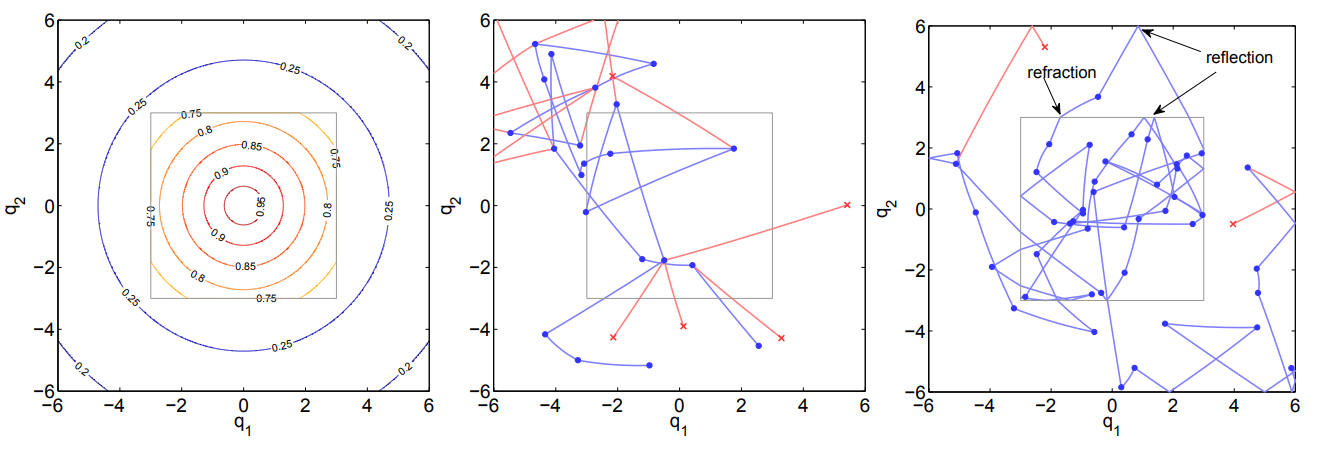
\includegraphics[width=0.9\textwidth]{publications/presentations/log_concave_sampling/reflection.png}
        \caption{Baseline and Reflective HMC. Taken from \cite{afshar2015reflection}.} 
        \label{fig:reflection}
    \end{figure}

\end{frame}

\begin{frame}[allowframebreaks]{The Reflection Operator}
    A point $x$ reflects at the boundary point $\tilde x$ with normal $n$.
    
    \medskip
    
    We define the reflection operator $\textrm{refl}$ such that 
    
    $$
    \textrm{refl}(x) = - 2 (a^T n) n + a + \tilde x
    $$

    where $a = \tilde x - x$ is the ray between the initial and the boundary points. Note that in general $\textrm{refl}(x)$ may not lie in $K$. We compose the reflection operator $k$ times such that $\textrm{refl}^k (x) = \mathrm {refl} \circ \dots \circ \mathrm{refl} (x) \in K$. In our setting we assume that at each step the proposal point cannot reflect more than $\ell \in \mathbb N^*$ times.

    \framebreak 
    
    \begin{figure}
        \centering
        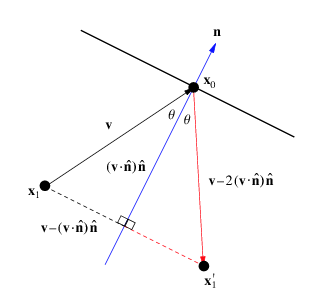
\includegraphics[width=0.4\textwidth]{publications/presentations/log_concave_sampling/reflection_w.png}
        \caption{Reflection Illustration. $x_1'$ is the reflection of $x_1$ about $x_0$ with normal $n$. Source: \url{https://mathworld.wolfram.com/Reflection.html}}
        \label{fig:my_label}
    \end{figure}
    
\end{frame}


\begin{frame}[allowframebreaks]{Computing Intersections with $\partial K$}
    
    
    Of particular interest is the computation of the intersection of an (implicit) curve between a point $x$ inside the convex body $K$ and a proposal $\tilde x \not \in K$. 
    
    \medskip

    \textbf{Case 1.} The curve is a \emph{line segment} and $K$ is a convex polytope.

    We parametrize the line segment between $x$ and $\tilde x$ with $\gamma(t) = t x + (1 - t) \tilde x$ where $t \in [0, 1]$. We seek $t_u = \sup \{ t \in [0, 1] | \gamma(t) \in \partial K \}$ and $u = \gamma(t_u)$ as the solution to the boundary intersection problem. 
    
    \medskip
    
    We use the Cyrus-Beck  \cite{cyrus1978generalized} algorithm
    
    \framebreak
    
    Let $z \in \partial K$ be known and let $n$ represent the normal vector at $z$. We compute the quantity 
    
    \begin{equation*}
        n^T (\gamma(t) - z) \begin{cases} = 0 & \gamma(t) \in \partial K \\
        < 0 & \gamma(t) \notin K \\
        > 0 & \gamma(t) \in K \setminus \partial K
        \end{cases}
    \end{equation*}

    Solving the equation $n^T (\gamma(t) - z)$ for $t$ we get 
    
    $$t = \frac {n^T (z - x)} {n^T (\tilde x - x)}$$

    We compute the above for all the $N$ normals of the polytope and keep the maximum value that lies in $[0, 1]$. The min value can also be kept in case we want the other intersetion point as well. Complexity is $O(Nd)$
    
    \framebreak
    
    \textbf{H-polytope.} The polytope is given by the form $Ax \le b$ where $A$ consists of $N$ row vectors $A_1, \dots, A_N \in \mathbb R^d$ and $b = (b_1, \dots, b_N)^T$. On each facet we use $A_i$ as normal vector and if $b_i = 0$ then we use $\vec 0$ as a point on the facet. If $b_i \neq 0$, there exists at least one index $r$ such that $A_{ir} \neq 0$ (otherwise the problem is trivial) we use the point $u = (0, 0, \dots, b_i / A_{ir}, \dots, 0)^T$ which lies on the hyperplane, that is $A_i^T u = b_i$. Worst-case complexity is $O(Nd)$. 
    
    \framebreak
    
    \textbf{V-polytope.} The polytope is given by its convex hull $V$ which contains $M$ points $v_1, \dots, v_M \in \mathbb R^d$. The point $\gamma(t) = tx + (1 -t) \tilde x$ is on the boundary for some $t_0 \in [0, 1]$ (given that $x \in K$) if $t_0$ is the maximum value of $t \in [0,1]$ such that there exist $\lambda_1, \dots, \lambda_M \ge 0$ with $\sum_{i  =1}^M \lambda_i = 1$ and $\gamma(t_0) = \sum_{i = 1}^M \lambda_i v_i$, which translates to the following LP problem which has $O(Md)$ constraints
    
    \begin{align*}
        \text{maximize} \quad & t & \\
        \text{subject to} \quad & 0 \le t \le 1 & \\
        & \lambda_i \ge 0 & i \in [M] \\
        & \sum_{i = 1}^M \lambda_i = 1 \\
        & t x + (1 - t) \tilde x - \sum_{i = 1}^M \lambda_i v_i = 0 
    \end{align*}
    
    Solvable via $\texttt{lp\_solve}$ (functionality already exists)
    
    \framebreak
    
    \textbf{Case 2.} The curve has the form $\gamma(t) = \sum_{i = 1}^m a_i \phi_i(t)$, $\{ \phi_j \}_{j \in [m]}$ are basis functions, and $K$ is a convex polytope.
    
    \medskip
    
    \textbf{H-polytope.} We use the same procedure as above, however now we cannot solve directly for $t$. We, for example, can use the Newton-Raphson root finder to solve the transcendental equation.
    
    \begin{equation*}
        t^{(r + 1)} = t^{(r)} - \frac {\sum_{j \in [m]} (n^T a_j) \phi_j(t^{(r)}) - n^T z } {\sum_{j \in [m]} (n^T a_j) \dot \phi_j(t^{(r)})}
    \end{equation*}

    Complexity is $O(NdRm)$ where $R$ is the maximum number of iterations the NR solver must be called to find a root. 
    
    \underline{Alternatively.} Solve optimization problem $\max_{t \ge 0} t$ subject to $A \gamma(t) \le b$. The constraint translates to $\tilde A \Phi \le b$ where $\Phi$ is a column vector that contains $\phi_j(t)$ and $\tilde A$ is the product of the matrix $A$ and the coefficient matrix. 
     
    \textbf{Problems.} Convergence, Well-posedness (denominator getting too small)

    \framebreak
    
    \textbf{V-polytope.} The problem of Case I is a general optimization problem 
    
    \begin{align*}
        \text{maximize} \quad & t & \\
        \text{subject to} \quad & t \ge 0 \\
        & \lambda_i \ge 0 & i \in [M] \\
        & \sum_{i = 1}^M \lambda_i = 1 \\
        & \sum_{i = 1}^M a_j \phi_j(t) - \sum_{i = 1}^M \lambda_i v_i = 0 
    \end{align*}
    

    Can be solved via interior-point-methods such as line-search filters (e.g. using the COIN-OR IPOPT toolbox)

    \framebreak
    
    \textbf{Case 3.} The convex body $K$ has the form $K = \{ x \in \mathbb R^d | g(x) \le 0 \}$ where $g(x) = \max_{1 \le i \le M} g_i(x)$ where $g_1, \dots, g_M$ are twice-differentiable convex functions that are $\mu$-strongly-convex. 
    
    \medskip
    
    \textbf{Examples.} $L_2$ Balls, Spectrahedra etc.
    
    \medskip
    
    \textbf{Idea.} Linearize the convex body around $x + h$
    
    $$0 \ge g_i(x + h) \ge g_i(x) + \langle \nabla g_i(x), h \rangle + \frac {\mu \| h \|^2}  2 $$
    
    The linearized convex polytope $P(x)$ around $x$ is 
    
    $$J(x) h \le b$$
    
    where $J(x)$ is the Jacobian matrix around $x$ with entries $J_{ij}(x) = \frac {\partial g_i(x)} {\partial x_j}$ and $b$ has entries $b_i = -g_i(x)$.
    
    \framebreak 
    
    The linear approximation error is at most $\frac {\mu} 2 \| h \|^2$.     A high-level algorithm (Local-search-based) proceeds as follows.
    
    \medskip

    We are given a curve $\gamma(t)$ and a starting point $x_0 = \gamma(0)$, an accuracy $\epsilon > 0$, and a step counter $i$ initialized at 0.
    
    \begin{enumerate}
        
        \item Find $P(x_i)$ around $x_i$ and the intersection point of $\gamma(t)$ with $P(x_i)$ (see Case 1, Case 2). Let that point be $x_{i + 1} = \gamma(t_{i + 1})$
        \item Calculate $g(x_{i + 1}) = \max_{1 \le j \le M} g_j(x_{i + 1})$. If $|g(x_{i + 1)}| \le \epsilon$, output $x_{i + 1}, t_{i + 1}$, else repeat. 
    \end{enumerate}
    
\end{frame}

\begin{frame}{Progress Report for GSoC}
 
    The working repository can be found here
    
    \begin{center}
        \url{https://github.com/papachristoumarios/volume_approximation}
    \end{center}
 
    What has been implemented (including testing and source code docs)
    
    \begin{enumerate}
    \item ODE Solvers (\texttt{include/ode\_solvers})
    \begin{enumerate}
        \item Euler Sovler
        \item RK Solvers (RK4, Midpoint, etc.)
        \item Leapfrog Solver
        \item Bulirsch–Stoer-Richardson Solver
        \item Collocation Method (ongoing)
    \end{enumerate}
    \item Research Paper (ongoing)
    \item Boundary Oracles curves of the form $\gamma(t) = \sum_j a_j \phi_j(t)$ (ongoing)
    \item Samplers: HMC with reflections 
    \end{enumerate}
 
    \textbf{Next Steps.} SDEs (Langevin), R bindings, more Documentation, more Testing 
    
    
\end{frame}


\begin{frame}{Next Talk(s)}

Next talk(s) will be occupied with 

\begin{enumerate}
    \item Algorithmic Issues for the sampling problem (mixing time, bounds etc.).
    \item Theoretical contributions to the problem.
    \item Implementation details.
\end{enumerate}
    
\end{frame}


\begin{frame}{}
    \vfill
    \centering
    \Huge {
        \textbf{Thank you!}
    }
    \vfill
\end{frame}



\begin{frame}[allowframebreaks]{References}
    \small {

    \bibliographystyle{alpha}
    \bibliography{references}
    
    }
\end{frame}


\end{document}

